\documentclass[a4paper,10pt]{article}
\usepackage[pdftex]{graphicx}
\newcommand{\HRule}{\rule{\linewidth}{0.5mm}}
\usepackage{greektex}
\usepackage{hyperref}
\usepackage{listings}
\usepackage{wrapfig}
\usepackage{graphicx}
\usepackage[usenames,dvipsnames]{color}
\usepackage[table]{xcolor}
%--------Footers-Headers---------------
\usepackage{fancyhdr}
\pagestyle{fancy}
\fancyhead[LE,RO]{\slshape \rightmark}
\fancyhead[LO,RE]{\slshape \leftmark}
\fancyfoot[C]{\thepage}
%-----Greek language-----------------
\usepackage[cm-default]{fontspec}
\usepackage{xunicode}
\usepackage{xltxtra}
\usepackage{amsmath}
\usepackage{xgreek}
%-----Fonts-------------------------
\setromanfont{FreeSerif}
\setsansfont{FreeSans}
\setmonofont{FreeMono}
%----------Hyper linking setup----------------
\hypersetup{
    bookmarks=false,         % show bookmarks bar?
    unicode=true,          % non-Latin characters in Acrobat’s bookmarks
    pdftoolbar=false,        % show Acrobat’s toolbar?
    pdfmenubar=false,        % show Acrobat’s menu?
    pdffitwindow=false,     % window fit to page when opened
    pdfstartview={FitH},    % fits the width of the page to the window
    pdftitle={My title},    % title
    pdfauthor={Author},     % author
    pdfsubject={Subject},   % subject of the document
    pdfcreator={Creator},   % creator of the document
    pdfproducer={Producer}, % producer of the document
    pdfkeywords={keyword1} {key2} {key3}, % list of keywords
    pdfnewwindow=true,      % links in new window
    colorlinks=true,       % false: boxed links; true: colored links
    linkcolor=black,          % color of internal links
    citecolor=green,        % color of links to bibliography
    filecolor=magenta,      % color of file links
    urlcolor=blue           % color of external links
}
%----------code setup----------------
\lstset{language=verilog,
   keywords={module,initial,forever,begin,wait,case,else,elseif,end,for,function,
      if,assign,while,always,or,posedge,endmodule},
   keywordstyle=\bfseries\color{BrickRed},
   keywords=[2]{wire,input,output,reg},
   keywordstyle={[2]\bfseries\color{OliveGreen}},
   basicstyle=\footnotesize,
   commentstyle=\color{blue},
   stringstyle=\color{green},
   numbers=left,
   numberstyle=\tiny\color{black},
   stepnumber=1,
   numbersep=5pt,
   backgroundcolor=\color{Goldenrod},
   tabsize=5,
   showspaces=false,
   frame=single,
   showtabs=false,
   showstringspaces=false} 

%---------image border--------
\usepackage{float}
\floatstyle{boxed} 
\restylefloat{figure}


%opening
%\title{\bf ΛΟΓΙΚΗ ΣΧΕΔΙΑΣΗ 2}
%\author{  Καλάργαρης Χαράλαμποs, AM:3929 \and  Καλάργαρης Χαράλαμποs, AM:3929 \and   Καλάργαρης Χαράλαμποs, AM:3929 }
%\date{27/5/2011}

\begin{document}
\begin{titlepage}

\begin{center}


% Upper part of the page

\includegraphics[width=0.25\textwidth]{/home/federico/Documents/Kile/Diploma/Front_Page/ceid.png}\\[1cm]    
%%/home/federico/Pictures/appmakr-logo.png
\textsc{\LARGE Πανεπιστημίο Πατρών}\\[1.5cm]

\textsc{\Large Μηχανικών Η/Υ και Πληροφορικής}\\[2.5cm]


% Title
\HRule \\[0.4cm]
{ \Large \bfseries Σχεδιασμός System-on-Chip για επεξεργασία εικόνας και υλοποίηση με FPGA. }\\[0.4cm]

\HRule \\[3.5cm]

% Author and supervisor
\begin{minipage}{0.4\textwidth}
\begin{flushleft} \large
\emph{Author:}\\
Χαράλαμπος \textsc{Καλάργαρης}
\end{flushleft}
\end{minipage}
\begin{minipage}{0.4\textwidth}
\begin{flushright} \large
\emph{Supervisor:} \\
Θεμιστοκλής \textsc{Χανιωτάκης}
\end{flushright}
\end{minipage}

\vfill

% Bottom of the page
{\large \today}

\end{center}

\end{titlepage}
%\maketitle
\newpage
\tableofcontents
\newpage
\listoffigures
\newpage

\section{Εισαγωγή}
{
}

\section{OpenRISC Family}
{Η OpenRISC 1000 οικογένεια επεξεργαστών αναφέρεται σε μια ελεύθερη, ανοιχτού
λογισμικού RISC αρχιτεκτονική κεντρικών μονάδων επεξεργασίας.Σχετικά με την
αρχιτεκτονική, η OpenRISC 1000 οικογένεια στοχεύει σε ένα φάσμα υλοποιήσεων που	
ποικίλουν ως προς την τιμή/αποδοση και το είδος της εφαρμογής.Είναι μια 
32/64-bit φορτωσης και αποθήκευσης (load and store) RISC αρχιτεκτονική που σχεδιάστηκε
με έμφαση στην απόδοση, στην απλότητα, στην χαμηλή ενεργειακή κατανάλωση, στην επεκτασιμότητα
και στην ευελιξία.Η OpenRISC αρχιτεκτονίκη στοχεύει σε μεσσαία και υψηλή απόδοση
δικτύωσης (networking), σε ενσωματομένα, αυτοκινητοβιομηχανικά και φορητά υπολογιστηκά περιβάλλοντα.

\vspace{0.7cm}
\begin{figure}[h!]
 \centering
 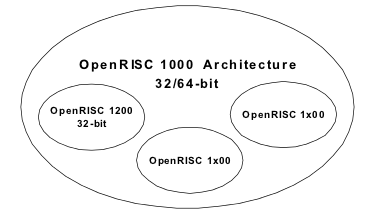
\includegraphics[bb=0 0 376 214,scale=0.7]{/home/federico/Documents/Kile/Diploma/Images/OR_family.png}
 % OR_family.png: 376x214 pixel, 72dpi, 13.26x7.55 cm, bb=0 0 376 214
 \caption{Σχηματική αναπαράσταση OpenRISC αρχιτεκτονικής.}
\end{figure}
\vspace{0.7cm}


Όλες οι OpenRISC υλοποιήσεις που το πρώτο ψηφίο στον αριθμό ταυτότητας
(identification number) ειναι '1' ανήκουν στην 
OpenRISC 1000 οικογένεια.Το δεύτερο ψηφίο ορίζει ποια χαρακτηριστικά της OpenRISC
1000 αρχιτεκτονικής είναι υλοποιημένα και με ποιο τρόπο είναι υλοποιημένα.Τα δύο
τελευταία ψηφία αναφέρονται στο πως μια υλοποιήση ηταν παραμετροποιημένη πριν 
χρησιμοποιηθει σε πραγματική εφαρμογή.
\subsection{OpenRISC 1200}
{ Ο OR1200 είναι ενας 32-bit βαθμωτός RISC επεξεργαστής με Harvard μικροαρχιτεκτονική,
5 stage integer pipeline, υποστήριξη εικονικής μνήμης (MMU) και βασικές δυνατότητες
DSP.

Οι προκαθορισμένες κρυφες μνήμες ειναι:
\begin{itemize}
 \item 1-way direct-mapped 8KB κρυφή μνήμη δεδομένων.
 \item 1-way direct-mapped 8KB κρυφή μνήμη εντόλων.
 \item Κάθε κρυφή μνήμη έχει γραμμή μεγέθους 16-byte.
 \item Και οι δύο κρύφές μνήμες ειναι  physically tagged(todo).
\end{itemize}

Η προκαθορισμένη MMU αποτελείται από:
\begin{itemize}
 \item 64-entry hash based 1-way direct-mapped data TLB.
 \item 64-entry hash based 1-way direct-mapped instruction TLB.
\end{itemize}

Μερικές άλλες επιπρόσθετες λειτουργίες που παρέχει ο OpenRISC 1200 ειναι η μονάδα
απασφαλμάτωσης πραγματικού χρόνου (real-time debug unit), υψηλής ανάλυσης χρονιστή,
προγραμματιζόμενο ελεκτή διακοπών (programmable interrupt controller) και μονάδα
ρύθμισης των ενεργειακών απαιτήσεων.


Ο OR1200 ουσιαστικά προορίζεται για εφαρμογες σε ενσωματομένα,φορητά και δικτύωσης
συστήματα.Μπορεί να ανταγωνιστεί τους τελευταίους βαθμωτούς 32-bit RISC επεξεργαστές
της κλάσης του και να υποστηρίξει αποδοτικά οποιοδήποτε μοντέρνο λειτουργικό σύστημα.
Ανταγωνιστές του θεωρούνται οι ARM10, ARC και Tensilica RISC επεξεργαστές.
\newline \newline
Παρακάτω βρίσκεται η σχηματική αναπαράσταση του OR1200 επεξεργαστή με τις υπομονάδες
που τον αποτελούν.

\begin{figure}[h!]
 \centering
 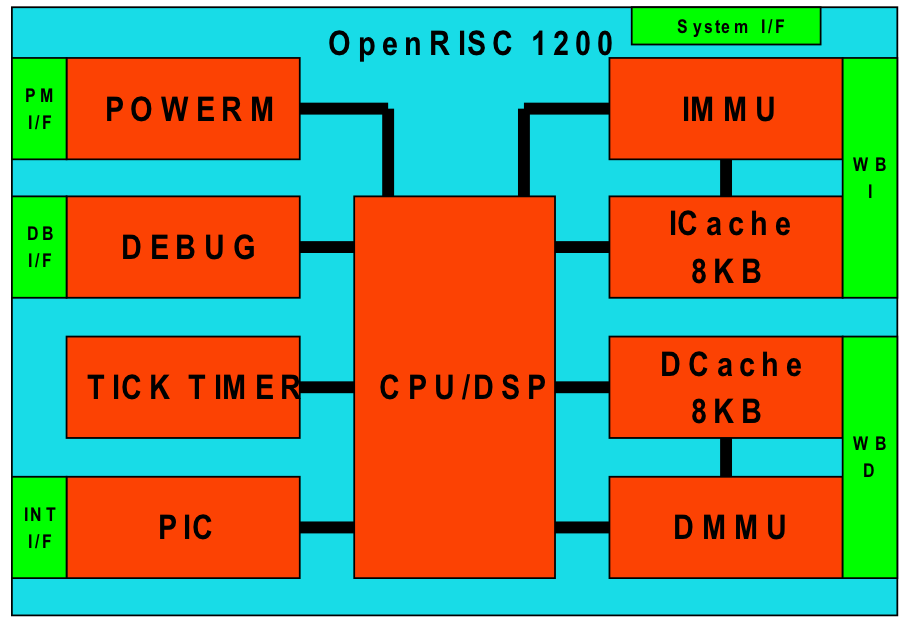
\includegraphics[bb=0 0 905 625,scale=0.3]{/home/federico/Documents/Kile/Diploma/Images/or1200.png}
 % or1200.png: 905x625 pixel, 72dpi, 31.93x22.05 cm, bb=0 0 905 625
 \caption{Core's Architecture}
\end{figure}

\begin{itemize}
 \item CPU/FPU/DSP central block.
 \item Direct-mapped data cache.
 \item Direct-mapped instruction cache.
 \item Data MMU based on hash based DTLB.
 \item Instruction MMU based on hash based ITLB.
 \item Power management unit and power management interface.
 \item Tick timer.
 \item Debug unit and development interface.
 \item Interrupt controller and interrupt interface.
 \item Instruction and Data WISHBONE host interfaces.
\end{itemize}
\begin{figure}[h!]
 \centering
 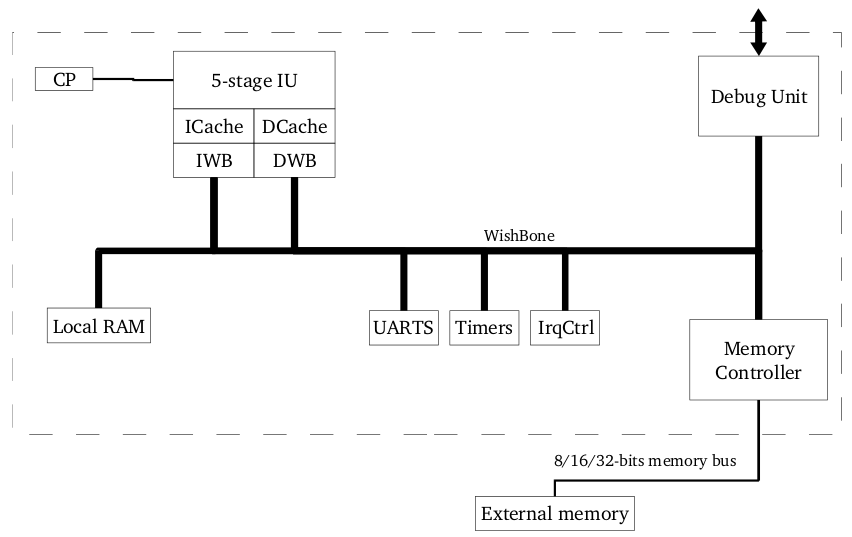
\includegraphics[bb=0 0 852 537,scale=0.4]{/home/federico/Documents/Kile/Diploma/Images/or1200eval.png}
 % or1200eval.png: 852x537 pixel, 72dpi, 30.06x18.94 cm, bb=0 0 852 537
 \caption{OR1200 Overview}
\end{figure}

Συνοπτικά παρουσιάζονται παρακάτω τα χαρακτηριστικά του OR1200:

{%
\newcommand{\mc}[3]{\multicolumn{#1}{#2}{#3}}
\definecolor{tcD}{rgb}{0.839216,0.92549,0.8}
\definecolor{tcA}{rgb}{0.498039,0.819608,0.231373}
\definecolor{tcB}{rgb}{0.847059,0.933333,0.807843}
\definecolor{tcC}{rgb}{0.87451,0.917647,0.858824}
\begin{center}
\begin{tabular}{ll}
% use packages: color,colortbl
\rowcolor{tcA}
  & \textbf{OR 1200}\\
\rowcolor{tcB}
\textbf{License} & \textit{GNU LGPL}\\
\rowcolor{tcC}
\textbf{Platform} & \textit{FPGA, ASIC}\\
\mc{1}{>{\columncolor{tcB}}l}{\textbf{Distributed file format}} & \mc{1}{>{\columncolor{tcD}}l}{\textit{Verilog}}\\
\rowcolor{tcC}
\textbf{General} &  \\
\rowcolor{tcD}
Architecture & \textit{32-bit RISC}\\
\rowcolor{tcC}
Byte Ordering & \textit{Big endian}\\
\rowcolor{tcD}
Pipeline depth & \textit{5}\\
\rowcolor{tcC}
Issue type & \textit{Single}\\
\rowcolor{tcD}
\textbf{Register file} &  \\
\rowcolor{tcC}
Organization & \textit{Flat}\\
\rowcolor{tcD}
\# of global registers & \textit{32}\\
\rowcolor{tcC}
Total \# of GPRs & \textit{32}\\
\rowcolor{tcD}
\textbf{ISA} &  \\
\rowcolor{tcC}
Type & \textit{ORBIS32}\\
\rowcolor{tcD}
Addressing modes & \textit{Immediate,
displacement, pcrelative}\\
\rowcolor{tcC}
MAC & \textit{32x32-bit, 48-bit Acc}\\
\rowcolor{tcD}
Custom instructions & \textit{Yes}\\
\rowcolor{tcC}
Custom coprocessor & \textit{Yes}\\
\rowcolor{tcD}
Software floating-point support & \textit{IEEE-754 Single and double precision}\\
\rowcolor{tcC}
\textbf{Cache} &  \\
\rowcolor{tcD}
Hierarchy & \textit{Harvard}\\
\rowcolor{tcC}
Instruction cache
size & \textit{512 byte-8 Kbyte}\\
\rowcolor{tcD}
Data cache size & \textit{4-8 Kbyte}\\
\rowcolor{tcC}
Line size & \textit{8-16 byte}\\
\rowcolor{tcD}
Placement scheme & \textit{Direct-mapped}\\
\rowcolor{tcC}
Valid bits & \textit{One per cache line}\\
\rowcolor{tcD}
Line-locking & \textit{Set basis}\\
\rowcolor{tcC}
\textbf{System Interface} & \textit{Wishbone SoC rev. B32-bit}\\
\rowcolor{tcD}
\textbf{Power Management} & \textit{Slow and idle mode, sleep mode, doze mode}\\
\rowcolor{tcC}
\textbf{Memory} &  \\
\rowcolor{tcD}
On-chip RAM & \textit{Configurable} \\
\rowcolor{tcC}
\textbf{Operating system
support} & \textit{Linux, uClinux, OAR RTEMS RTOS}\\
\end{tabular}
\end{center}

}%
\vspace{0.7cm}
}


}



\section{OR1200 Simulation}{

\subsection{Simulation Enviroment}{
Υπάρχουν δύο περιβάλλοντα με τα οποία γίνετε η εξομοίωση του OR1200 επεξεργαστή.
Το πρώτο χρησιμοποιεί τον OpenRISC αρχιτεκτονικό εξομοιωτή \emph{or1ksim} και 
το δεύτερο χρησιμοποιέι τον \emph{NC-Verilog} εξoμοιωτή που κάνει εξομοίωση με βάση
το υλικό (hardware based simulation).Στο πρώτο περιβάλλον γίνετε η επαλήθευση
της λειτουργικότητας των benchmarks και στο δεύτερο προσομοιώνεται η ουσιαστική
λειτουργία του OR1200 σε επίπεδο υλικού με βάση το benchmark που εκτελέσαμε.\newline


Η συνολική ροή της εξομοίωσης παρουσιάζεται στο Σχήμα 4.Τα benchmarks είναι 
είτε .C αρχέια είτε .S αρχεία.Αύτα τα αρχεία, αρχίκα γίνονται cross-compiled
 χρησιμοποιώντας την εντολή or32-uclinux-gcc και παράγουν ένα .O object αρχείο.
Το object αρχείο μετά μετατρέπεται σε ενα .OR32 εκτελέσιμο αρχείο χρησιμοποιώντας
την συνδετική εντολή or32-uclinux-ld. Αυτό το εκτελέσιμο αρχέιο χρησιμοποιείται
απο τον or1k αρχιτεκτονικό εξομοιωτή.Περαιτέρω το αρχείο .OR32 μετατρέπεται σε
δυαδικό (binary) αρχείο χρησιμοποιώντας την εντολή or32-uclinux-objcopy.Στο τέλος
δημιουργείται ενα .HEX αρχείο χρησιμοποιώντας τον binary to hex μετατροπέα
 bin2hex. Το παραγώμενο αρχείο .HEX φορτώνεται στην flash μνημη του RTL κώδικα
του OR1200 επεξεργαστή και μετά γινετε η εξομοίωση με βάση το υλικό.
 
\begin{figure}[h!]
 \centering
 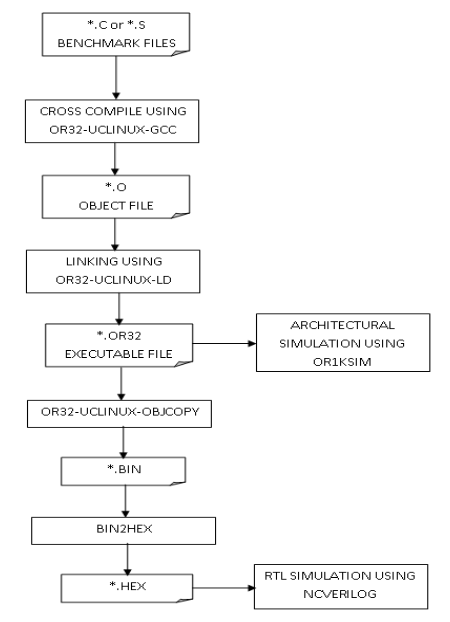
\includegraphics[bb=0 0 450 622,scale=0.5]{/home/federico/Documents/Kile/Diploma/Images/overall_flow.png}
 % overall_flow.png: 450x622 pixel, 72dpi, 15.88x21.94 cm, bb=0 0 450 622
 \caption{Συνολική ροή εξομοίωσης.}
\end{figure}


}



\subsection{Package Structure}{
Σε αυτό το μέρος θα παρουσιάσουμε την δομή και τα περιεχομενα του φακέλου που αποτελεί 
τον επεξεργαστή OR1200.

Το συγκεκριμένο πακέτο περιέχει:
\begin{itemize}
 \item \underline{{\bf Rtl}} : Εδώ βρίσκεται ο κώδικας verilog που περιγράφει σε υλικό τον επεξεργαστή OR 1200.
\item \underline{{\bf Boards}} : Περιέχει κατάλληλα αρχεία για να περάσεις τον OR1200 σε συγκεκριμένες πλακετες
FPGA.
\item \underline{{\bf Sim}} : Σε αυτό τον φάκελο δημιουργούνται τα αποτελέσματα της εξομοίωσης σύμφωνα με
το Makefile που δημιουργήσαμε για τους σκοπούς του εργαστηρίου. \begin{enumerate}
                                                                 \item \emph{sim/bin} : Εδώ βρίσκεται το Makefile που δημιουργήσαμε για τους σκοπούς του
εργαστηρίου και χειρίζεται την λειτούργια του επεξεργαστή.
                                                                 \item \emph{sim/run} :Εδώ εκτελούνται όλες οι εντολές που σχετίζονται με την εξομοίωση
του επεξεργαστη.
                                                                 \item \emph{sim/out} :Εδώ τοποθετούνται όλα τα αρχεία που παράγονται μετά την εξομοίωση.
Να σημειωθεί οτι τα waveforms τοποθετούνται στο sim/run.
                                                                \end{enumerate}

\item \underline{{\bf Sw}} : Εδω βρίσκονται τα βασικότερα αρχεία που είναι απαραίτητα για το cross-compilation 
και την σωστή λειτουργία του OpenRISC επεξεργαστή.
					  \begin{enumerate}
                                           \item \emph{sw/drivers} :Εδω βρίσκονται οι drivers και τα εργαλεία για τροποποίηση του hardware.
					   \item \emph{sw/lib} :Eδω βρίσκεται μια απλή βιβλιοθήκη που σε συνδυασμο με τους drivers κατά την διάρκεια του compile δημηιουργούν την βιβλιοθήκη liborpsoc 
που τοποθετείται στο \emph{sw/lib}.
					   \item \emph{sw/lib/include} :Εδώ βρίσκεται το αρχείο cpu-utils.h που περιέχει όλες τις συναρτήσεις σχετίκες
με την CPU του OpenRISC.
					   \item \emph{sw/tests} :Εδώ βρίσκεται το λογισμικό που χρησιμοποιείται (.C και .S αρχέια) για να δοκιμαστεί η σωστή λειτουργία
του επεξεργαστή (testing) σε υπομονάδες οπως ethmac, or1200,sdram, spi και uart.Στον φάκελο κάθε υπομονάδας (πχ sw/test/sdram) υπάρχουν δύο υποφάκελοι board 
και sim (πχ sw/test/sdram/board και sw/test/sdram/sim).Στον sim φάκελο υπαρχουν τα tests που εκτελούνται κατα την εξομοίωση του επεξεργαστη σε ενα PC και στον
φάκελο board υπάρχουν τα tests που εκτελούνται κατά την λειτουργία του επεξεργαστή.
                                          \end{enumerate}

\item \underline{{\bf Doc}} : Εδω βρισκεται documentation που χρειαζόμαστε για να καταλαβουμε την φύση των
testbenches και οι οδηγιες για το simulation συμφωνα με το Makefile που δημιουργησαμε για τους σκοπους του εργαστηρίου.
\end{itemize}
}



\subsection{Simulation commands}{
{
\subsubsection{ Η βασική διαδικασία}
{

Η διαδικασία με την οποία γίνετε η εξομοίωση του OR1200 είναι η εξής:
\begin{enumerate}
 \item Το Makefile που ελέγχει το simulation βρίσκετε στο \emph{/sim/bin/} και είναι προσπελάσιμο και απο το \emph{/sim/run/} .
 \item Στον φάκελο \emph{/sim/run/} εκτελώντας την εντολή \emph{make rtl-tests} κανει compile τον rtl
(verilog) κωδικα του OR1200 και εκτελεί όλα τα testbenches (assembly) που βρίσκονται στο \emph{sw/tests/or1200}.
 \item Tα αποτελέσματα του παραπάνω βήματος τοποθετούνται στο \emph{/sim/out/}. Aυτα ειναι (στα αγγλίκα για καλύτερη κατανόηση):
    \begin{itemize}
     \item \emph{test-name-executed.log} : A trace of the processor after each executed instruction
     \item \emph{test-name-sprs.log} : A list of processor special purpose registers (SPR) accesses is created
     \item \emph{test-name-lookup.log} : A list of when each instruction was executed is generated
     \item \emph{test-name-general.log} : The use of the processor’s report mechanism is commonplace in the
test software, as it allows for the checking of intermediate values after simulation.
    \end{itemize}
\end{enumerate}
}

\subsubsection{ Εκτέλεση ενος συγκεκριμένου test}
{

Η εξομοίωση ενός συγκεκριμένου test γίνετε με την εντολή
\emph{make rtl-test TEST=test-name\footnote{test-name: Είναι η ονομασία του test που θέλουμε να εκτελέσουμε.}} .Πρέπει το αρχείο \emph{test-name.c}
 (ή \emph{test-name.s} )να είναι τοποθετημένο στο \emph{sw/tests/module /sim/ } όπου module ειναι η υπομονάδα που θέλουμε να ελέξουμε με κάποιο απο τα tests που μας παρέχει 
(πχ sw/tests/sdram/sim/sdram-rows.c).
}

\subsubsection{Εκτέλεση συγκεκριμένων tests μαζί}
{

Η εξομοίωση πολλών συγκεκριμένων tests γίνετε με την εντολή \emph{make rtl-test TEST=" test-name1 test-name2 ..."} (πχ make rtl-tests TESTS="sdram-rows uart-simple or1200-mmu or1200-fp")
}


\subsubsection{ Παρέχοντας μια προσαρμοσμένη VMEM εικόνα (image)}
{

Είναι δυνατό να καθορίσουμε το μονοπάτι μιας ήδη υπάρχουσας VMEM εικόνας που θα την
χρησιμοποιήσουμε αντί να κάνουμε πάλι απο την αρχή test το software.Χρησιμοποιώντας
την μεταβλητή \emph{USER\_VMEM} μπορούμε να καθορίσουμε το μονοπάτι της VMEM εικόνας
που θέλουμε να τρέξουμε. Για παράδειγμα \emph{make rtl-test USER\_VMEM=/path/to/myapp.vmem}
Αυτή η εικόνα θα αντιγραφεί στο φάκελο στον οποίο εργαζόμαστε και θα μετονομαστέι
σύμφωνα με το τι η μνήμη στην εξομοίωση απαιτεί.
}

\subsubsection{ Παρέχοντας ένα "precompiled" εκτελέσιμο .ELF αρχέιο}
{

Είναι δυνατό να καθορίσουμε το μονοπάτι ενός OR32 ELF εκτελέσιμου αρχείου που θα το
χρησιμοποιήσουμε αντί να κάνουμε πάλι απο την αρχή test το software.Χρησιμοποιώντας
την μεταβλητή \emph{USER\_ELF} μπορούμε να καθορίσουμε το μονοπάτι στο οποίο βρίσκετε
αυτό το αρχείο. Για παράδειγμα \emph{make rtl-test USER\_ELF=/path/to/myapp.elf}
Το ELF αρχείο θα μετατραπεί σe δυαδίκη μορφή και μετά σε VMEM και θα φορτωθεί στο
μοντέλο για να εκτελεστέι.
}


\subsubsection{ Κυματομορφές}
{

Παράλλημα με το simulation ενός ή περισσοτέρων testbench παράγονται και οι κυματομορφές
των εξομοιώσεων που μας βοηθάνε στην καλύτερη κατανόηση τους.Τα αρχεία που παράγονται
βρίσκονται σε φακέλους μέσα στο \emph{/sim/run/} που έχουν την ονομασία \emph{test-name.shm} .Για να
εμφανίσεις τις κυματομορφές αυτές πρέπει μέσω κονσόλας να οδηγηθείς στο /sim/run/ και
μετά να εκτελέσεις την εντολή \emph{simvision test-name.shm}.
}

\subsubsection{ Eπιπρόσθετα επιλογές στις εντολες}
{

Παρακάτω παρουσιάζονται μερίκες μεταβλητές που μας βοηθούν να επιλέξουμε καποιές
συγκεκριμένες λειτουργίες.
\begin{itemize}
 \item \emph{END\_TIME    :}Αναγκάζει την εξομοίωση να τερματίσει (\$finish).Πχ 
\emph{make rtl-test TEST="or1200-mul" END\_TIME=100} όπου είναι ίδιο με το \emph{\#100 \$finish} σε αρχείο verilog.
\item \emph{DISABLE\_PROCESSOR\_LOGS    :} Απενεργοποιεί την οθόνη παρακολούθησης του επεξεργαστή
που συλλέγει πληροφορίες κατα την εκτέλεση μιας εξομοίωσης .Αυτό βοηθάει στην επιτάχυνση της εξομοίωσης αφού απαιτείται λιγότερος χρόνος στην
εγραφή αρχείων και αποτρέπει την δημιουργία πολύ μεγάλων αρχείων σε χρονοβόρες εξομοιώσεις.
\item \emph{SIMULATOR    :}Επιλέγουμε τον εξομοιωτή υλικου που θέλουμε να χρησιμοποιήσουμε.
Προκαθορισμένος εξομοιωτής ειναι ο NC-Verilog.Άλλη επιλόγη ειναι το ICARUS.
\end{itemize}

}
}
}

\end{document}